\subsection{Backward Stepwise Selection}

The second method applied is the dual of the previous one, i.e. \textit{Backward Stepwise Selection}. The model obtained is shown in figure \Fig~\ref{fig:BackwardModelSummary}.
\begin{figure}[h]
	\centering
	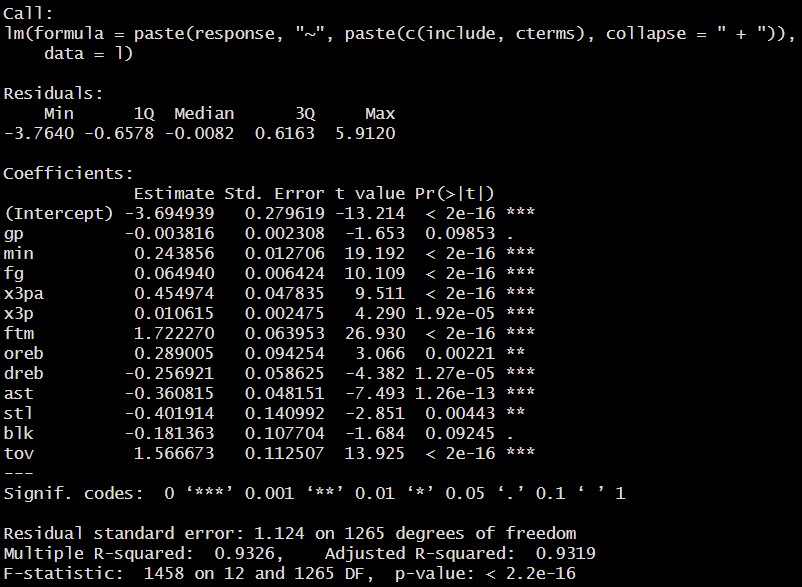
\includegraphics[width=0.4\linewidth]{ImageFiles/Regression/Backward/BackwardModelSummary}
	\caption{Backward Stepwise Selection Output Model.}
	\label{fig:BackwardModelSummary}
\end{figure}

The model obtained with this algorithm includes 12 variables, one less than Forward Stepwise. By comparing the two models it is possible to see that they have the same variables, except that Forward Stepwise included in addition \textit{"3P MADE"}, that was highly not significant. Therefore all the considerations made previously still hold.

However, removing the non significant variables the two models obtained by the two algorithms are the same, suggesting that the selection is good.